\chapter{Desenvolvimento}

O projeto foi desenvolvido na linguagem de programação C++ utilizando o \textit{framework} Qt para a parte gráfica e algumas de suas classes de geometria. A sua arquitetura foi feita de forma modular, composto por vários módulos que se comunicam entre si. Ele foi feito dessa forma para que caso futuramente surja a necessidade de se modificar alguma parte dele, como por exemplo trocar o motor gráfico ou utilizar um outro tipo de rede neural, isso possa ocorrer sem grandes dificuldades. Os três módulos principais que compõem o sistema são: algoritmo genético, simulador e rede neural artificial (RNA).

\begin{figure}[H]
    \caption{\label{img:blocos_alto_nivel}Representação de alto nível do sistema}
	\begin{center}
        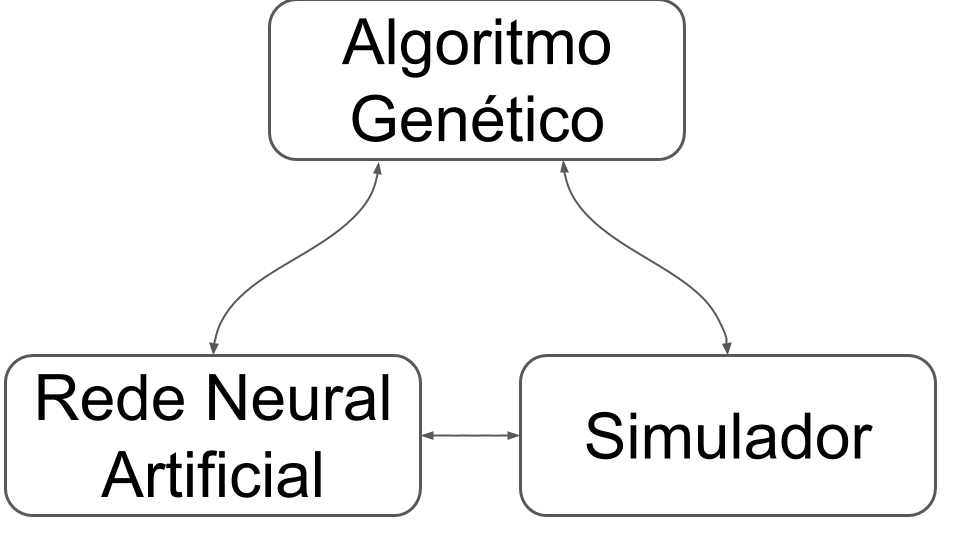
\includegraphics[scale=0.23]{img/blocos_principais.png}
	\end{center}
	\legend{Fonte: Elaborada pelo autor}
\end{figure}

Esses três módulos que podem ser observados na \autoref{img:blocos_alto_nivel} trocam informações entre si e agem um sobre o outro, onde o simulador representa um campo de futebol com robôs, a RNA controla os robôs do simulador e o AG realiza o treinamento da RNA otimizando os pesos de seus neurônios. O AG utiliza o simulador durante a etapa de treinamento da RNA.

\section{Simulador}

Foi desenvolvido um simulador dos robôs da categoria \textit{IEEE Very Small Size}. Os robôs do simulador estão em um campo com uma bola e todas as medidas de tamanho utilizadas estão de acordo com o manual de regras da competição \textit{IEEE Very Small Size Soccer} (VSSS) \cite{IEEE2008}.

O propósito principal do simulador é de ser utilizado no treinamento de um algoritmo genético, na função de aptidão durante a etapa de classificação das diferentes IAs. Portanto foi feito um esforço para o código ser eficiente em termos de processamento e memória, e de ser fácil de se interfacear com outras partes do sistema.

O simulador possui duas classes internas que são seus componentes mais básicos e importantes: \textit{Robo} e \textit{Bola}. Essas classes possuem funções e variáveis que controlam os parâmetros internos, como posição e velocidade por exemplo, assim como identificam o id de cada robô e para qual time ele está jogando. Ponteiros para objetos dessas classes são compartilhados entre as classes \textit{Fisica}, \textit{Grafico} e \textit{Interface}, de forma que todos eles apontem para a mesma variável, permitindo assim que essas três classes atuem e leiam as informações do robô e da bola sem a necessidade de consumir memória e processamento passando valores de uma classe para outra.

O simulador foi desenvolvido em dois módulos principais: física e gráfico. O módulo física é responsável pelos cálculos de colisões e movimentação dos robôs e da bola. O módulo gráfico é responsável pela exibição gráfica para o usuário do resultado da simulação.

A comunicação entre os módulos física e gráfico se dá por ponteiros de objetos da classe \textit{Bola} e \textit{Robo} que são compartilhados entre eles. O intuito dessa subdivisão em dois módulos é para que, caso no futuro se deseje utilizar outro \textit{framework} para a parte gráfica do simulador, ou se deseje utilizar alguma engine física no simulador, essa mudança não seja muito trabalhosa e possa ser feita só alterando as funções dentro do respectivo módulo.

Outra motivação para o desenvolvimento modular do simulador, o dividindo entre simulação física e exibição gráfica, é para aumentar a sua performance durante o treinamento do algoritmo evolutivo. Esses dois módulos são completamente separados e funcionam independente um do outro, deste modo se torna possível fazer a simulação dos robôs e se obter os resultados da partida ou mesmo gravar ela em um arquivo, sem consumir recursos de processamento para a exibir graficamente. Fazendo a simulação desse modo, se consegue focar todo o processamento do computador na simulação em si e ela fica muito mais rápida.

\begin{figure}[H]
    \caption{\label{img:simulador_blocos}Representação em blocos do simulador com as suas principais classes}
	\begin{center}
        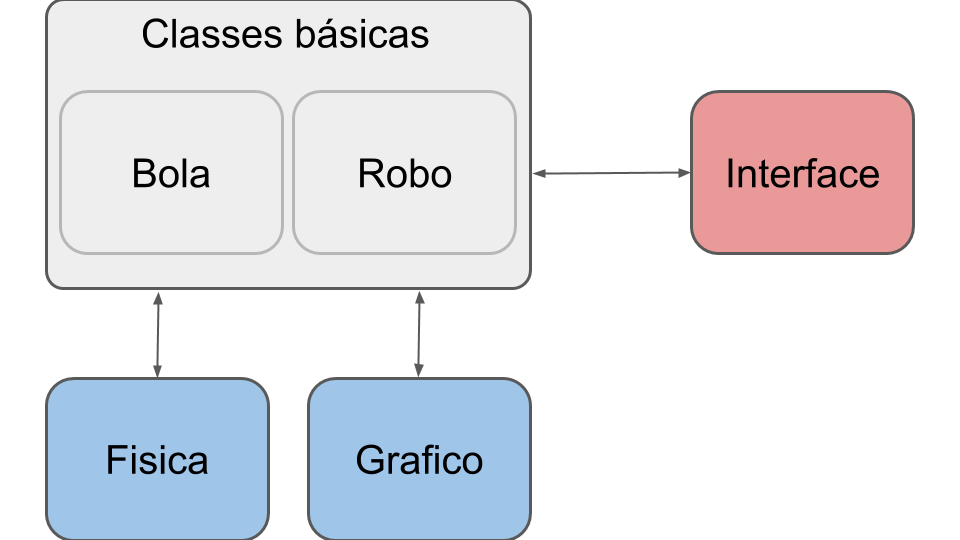
\includegraphics[scale=0.3]{img/sim_blocos.png}
	\end{center}
	\legend{Fonte: Elaborada pelo autor}
\end{figure}

\subsection{Exibição Gráfica}

O módulo responsável pela exibição gráfica do que está acontecendo no simulador, para que se possa acompanhar a movimentação dos robôs e da bola e fazer uma análise visual do comportamento da IA está implementado dentro da classe \textit{Grafico}. Esse módulo não é necessário para nada além da exibição gráfica, não alterando o valor de nenhuma variável importante do sistema.

A classe \textit{Grafico} possui internamente ponteiros para objetos da classe \textit{Robo} e \textit{Bola} e possui uma função de atualização importante que deve ser implementada obrigatoriamente, assim como a classe \textit{Fisica}. Essa função de atualização, sempre que chamada, atualiza a interface gráfica com as ultimas posições de cada robô e da bola.

A interface gráfica foi desenvolvida utilizando o \textit{framework} Qt , mas se por algum motivo for desejado alterar a ferramenta utilizada para fazer a interface gráfica, é necessário fazer duas modificações dentro da classe \textit{Grafico}. A primeira é modificar a função de atualização da classe \textit{Grafico}, essa função sempre que chamada deve atualizar a posição dos robôs e da bola na tela a partir dos valores de posição nas variáveis internas dos ponteiros para objetos da classe \textit{Robo} e \textit{Bola} que ela possui. A segunda modificação é alterar o construtor da classe gráfico, para receber os ponteiros para objetos da classe \textit{Robo} e \textit{Bola}, que são compartilhados com a classe \textit{Fisica}, e para inicializar a interface gráfica.

\begin{figure}[!htb]
    \caption{\label{img:sim_campo}Interface gráfica do simulador com dois times de robôs e uma bola laranja no meio do campo}
	\begin{center}
        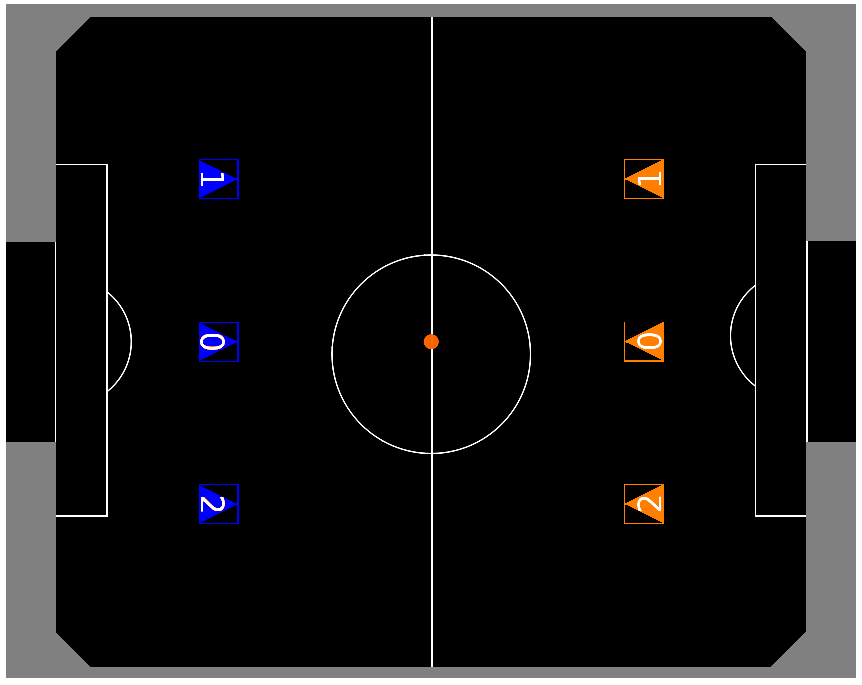
\includegraphics[scale=0.38]{img/sim_campo.png}
	\end{center}
	\legend{Fonte: Elaborada pelo autor}
\end{figure}

Na \autoref{img:sim_campo} está uma imagem gerada pela interface gráfica do simulador. Nela constam seis robôs, onde a cor deles representa o seu time, e cada robô possui uma numeração de identificação utilizada para diferenciar cada robô em relação aos outros de seu time. O ponto laranja no centro do campo é a bola e a linha branca desenhada dividindo o campo em dois, o circulo no meio e as formas próximas aos gols são apenas para fins de demarcação visual das partes do campo.

\subsection{Simulação Física}

O módulo responsável pelos cálculos de colisão entre os robôs, a bola e o campo, assim como o cálculo da trajetória e movimentação de cada robô e da bola está implementado dentro da classe \textit{Fisica}. Essa classe possui internamente ponteiros para objetos da classe \textit{Robo} e \textit{Bola} e possui uma função de atualização importante que deve ser implementada obrigatoriamente. Essa função, sempre que chamada, atualiza a posição e velocidades de cada robô e da bola realizando todos os cálculos de colisão e movimentação necessários para isso.

Como o objetivo primário do simulador é conseguir simular o mais rápido possível uma partida, a precisão da simulação foi comprometida e recursos como a derrapagem dos robôs e algumas outras situações específicas, não funcionam exatamente como na vida real. Isso foi feito de forma proposital e a proposta é utilizar esse simulador como uma ferramenta para o pré treinamento das IAs, que seria a fase do treinamento que exigiria mais recursos computacionais e iria desde uma IA sem treinamento algum, até alguma IA que já consegue desenvolver a sua função com esse simulador. O próximo passo seria desenvolver um simulador mais preciso, mesmo que ele exija mais recursos computacionais, e utilizá-lo para treinar uma IA pré treinada, como um ajuste fino antes de utilizar a IA com robôs reais.

Para o desenvolvimento de um simulador mais preciso, ou mais adequado para qualquer outra aplicação futura em que ele venha a ser utilizado, basta alterar a classe \textit{Fisica} implementando dentro da função de atualização as chamadas para outras funções ou realização de cálculos que atualizem os valores das variáveis de posição e velocidade dos robôs e da bola da forma que for desejado.

\begin{figure}[!htb]
    \caption{\label{img:campo_indicacao}Indicação da posição dos gols e traves, onde (A) representa a área do gol esquerdo e (B) representa as traves do gol direito}
	\begin{center}
        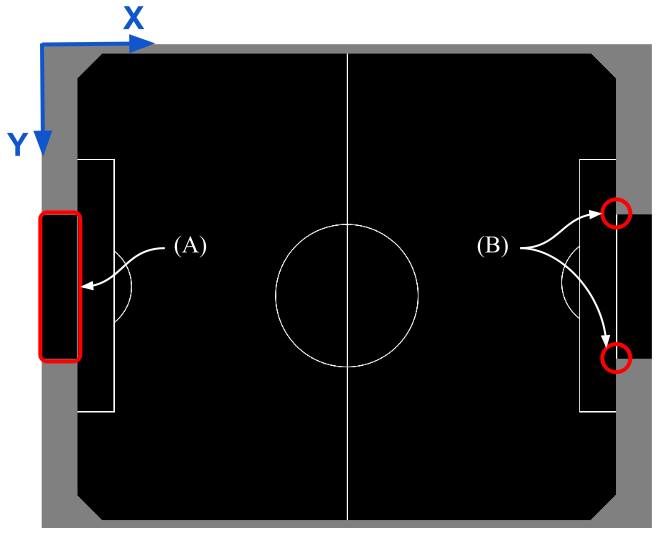
\includegraphics[scale=0.55]{img/campo_indicacoes.png}
	\end{center}
	\legend{Fonte: Elaborada pelo autor}
\end{figure}

O campo em que o robô está no simulador, representado na \autoref{img:campo_indicacao} possui uma superfície em preto pela qual os robôs e a bola podem se mover livremente, e em volta dessa superfície há uma parede representada pela cor cinza. A colisão do robô com a parede ou laterais de outros robôs faz com que ele cesse o seu movimento impedindo que ele se mova sobre essas superfícies. A interação da bola com a lateral dos robôs ou a parede faz com que ela, ao se chocar com a superfície, se mova da forma indicada na \autoref{img:reflexao_bola}, onde o ângulo de incidência e o ângulo de retorno são iguais.

\begin{figure}[!htb]
    \caption{\label{img:reflexao_bola}Comportamento da bola ao colidir com uma superfície}
	\begin{center}
        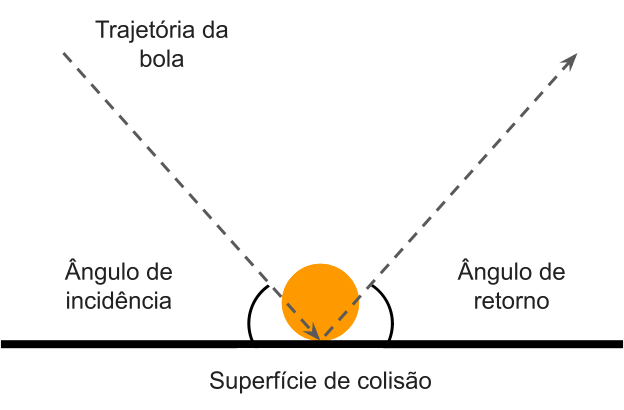
\includegraphics[scale=0.55]{img/colisao_bola.png}
	\end{center}
	\legend{Fonte: Elaborada pelo autor}
\end{figure}

Todos as posições de objetos representadas no simulador possuem dois valores, um é a componente de posição no eixo X e o outro é a componente de posição no eixo Y. O eixo X e Y está representado na \autoref{img:campo_indicacao} no seu canto superior esquerdo. Outras informações como velocidade por exemplo, também são calculadas considerando essa base.

O robô é definido por 5 pontos, um no seu centro, e outros quatro, um em cada vértice de um quadrado de lados iguais, além disso ele possui uma face que é considerada a frente do robô. Os robôs possuem dois graus de liberdade para movimentação: movimentação linear e movimentação angular. A movimentação linear permite que o robô se mova linearmente para frente e para trás (considerando a face da frente do robô). A movimentação angular permite que o robô rotacione com eixo no seu ponto central. A \autoref{img:robo_fisica} mostra os pontos que definem o robô e seus dois graus de liberdade. 

\begin{figure}[!htb]
    \caption{\label{img:robo_fisica} Representação de como o robô é visto pela simulação física. Os pontos vermelhos são os pontos que representam o robô e as setas são os seus graus de liberdade. A face superior do robô nessa imagem é a sua face frontal}
	\begin{center}
        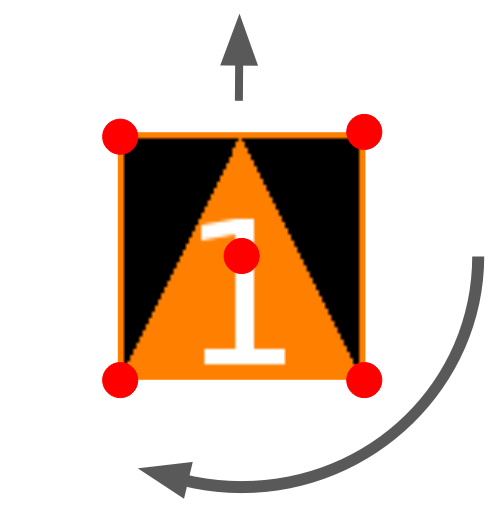
\includegraphics[scale=0.4]{img/robo_fisica.png}
	\end{center}
	\legend{Fonte: Elaborada pelo autor}
\end{figure}

\subsubsection{\label{cap:calc_colisao}Cálculo de colisão}

Primeiramente é necessário se definir o que é considerado uma colisão. Como que o algoritmo atua a intervalos de tempo discretos, muitas vezes a posição é calculada após a colisão já ter de fato ocorrido, por conta disso, é considerado a colisão de um ponto com uma reta o primeiro momento calculado pelo algoritmo em que o ponto atravessa a reta.

Para se detectar as colisões que podem ocorrer na simulação física, foram utilizadas três técnicas diferentes: comparar os valores de coordenas puros dos objetos, determinar de qual lado um ponto está em relação a uma reta, e determinar se um ponto se encontra dentro de um quadrado. Essas técnicas serão melhor explicadas a seguir.

\begin{alineas}[leftmargin=0pt, itemindent=20pt, labelwidth=15pt, labelsep=5pt, listparindent=1.25cm, align=left]
    \item Determinar colisão por comparação de posição.
    
    Este é o método mais simples de se detectar a colisão, porém no o simulador ele só pode ser aplicado para a colisão de um ponto com uma reta horizontal ou vertical. Para o caso de uma reta horizontal, é necessário saber a posição em X que ela começa e a que ela termina, e também é necessário saber a sua posição em Y. Se a posição em X do ponto for maior que a posição em X inicial da reta e menor que a posição em X final da reta, significa que o ponto está em condições de colidir com a reta. Se cumprido o requisito de estar em condições de colidir com a reta, o próximo passo é comparar a posição em Y do ponto com a posição em Y da reta. Se essa posição do ponto era menor que a da reta no momento anterior, e no próximo momento ela passou a ser maior que a da reta, então houve uma colisão. O mesmo ocorre para caso a posição fosse maior no momento anterior e no próximo passou a ser menor. Para o caso da reta ser vertical, o cálculo de colisão é feito da mesma maneira, porém invertendo os eixos X e Y.
    
    \begin{figure}[!htb]
        \caption{\label{img:colisao_simples}Exemplo de colisão por comparação de posição de um ponto com uma reta horizontal. A posição X inicial é representada por $x_i$, a posição X final é representada por $x_f$ e a posição em Y da reta é representada por $y_i$}
    	\begin{center}
            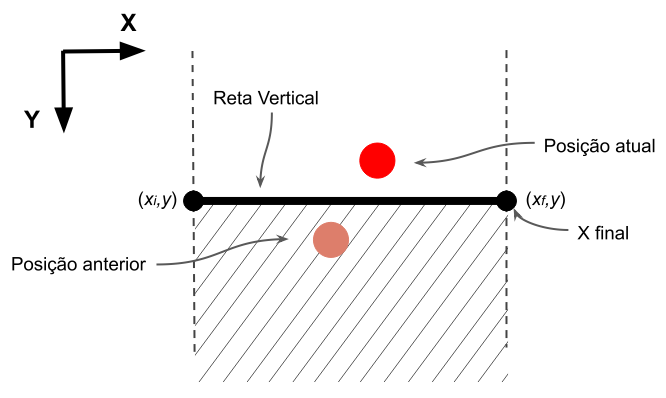
\includegraphics[scale=0.7]{img/colisao_simples.png}
    	\end{center}
    	\legend{Fonte: Elaborada pelo autor}
    \end{figure}
    
    \item Determinar de qual lado um ponto está em relação a uma reta.
    
    Esta técnica, em relação à técnica anterior, requer mais tempo de processamento, porém ela permite que o algoritmo determine de qual lado um ponto está em relação a uma reta, e por consequência descobrir se o ponto mudou de um lado para o outro da reta utilizando esta técnica em dois momentos diferentes, para uma reta com qualquer inclinação, e não apenas para uma reta vertical ou horizontal.
      
    \begin{figure}[!htb]
        \caption{\label{img:ponto_linha}Reta e ponto genéricos para cálculo de colisão}
    	\begin{center}
            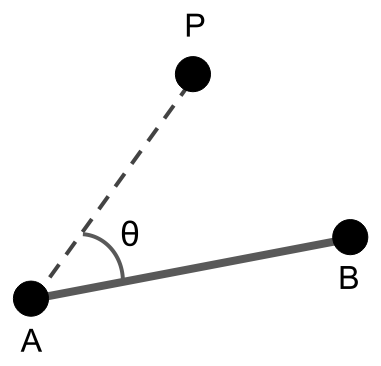
\includegraphics[scale=0.45]{img/ponto_linha.png}
    	\end{center}
    	\legend{Fonte: Elaborada pelo autor}
    \end{figure}
    
    Na \autoref{img:ponto_linha} observa-se uma reta $\overline{AB}$ definida pelos pontoa A e B, e um ponto P. Para se determinar de que lado da reta o ponto está, primeiro deve-se definir uma orientação para a reta, se a orientação da reta for definida no sentido de A para B, pode-se representar esta reta pelo vetor $\overrightarrow{AB}$ e o ângulo entre $\overrightarrow{AB}$ e $\overrightarrow{AP}$ é $\theta$. É calculado então o produto vetorial do vetor $\overrightarrow{AB}$ com o vetor $\overrightarrow{AP}$, dado pela \autoref{eq:produto_vetorial}, onde $\hat{k}$ é um vetor unitário perpendicular ao plano em que estão os ponto A, B e P.
    
    \begin{equation}
        \label{eq:produto_vetorial}
        \overrightarrow{AB} \times \overrightarrow{AP} = \hat{k} \, \norm{\overrightarrow{AB}} \, \norm{\overrightarrow{AP}}\ \, sen(\theta)
    \end{equation}
   
    Se o módulo do produto vetorial calculado $\norm{\overrightarrow{AB} \times \overrightarrow{AP}}$ for maior do que 0, o ponto P está acima da reta $\overline{AB}$ (tomando-se por referência o exemplo da \autoref{img:ponto_linha}), se ele for menor do que 0, ele está abaixo da reta, e se ele for igual a 0, ele está na reta. Isso ocorre pois como: $\norm{\overrightarrow{AB}} >= 0$ e $\norm{\overrightarrow{AP}} >= 0$, quem vai determinar o sinal do produto é o $sen(\theta)$, que é sempre maior do que zero para $\theta > 0^o$ (ponto P do lado de cima da reta) e é sempre menor do que zero para $180^o < \theta < 360^o$ (ponto P do lado de baixo da reta).
    
    \item Determinar se um ponto se encontra dentro de um quadrado.
    
    Utilizando-se a técnica de se determinar de qual lado um ponto está em relação a uma reta é possível de se determinar se um ponto se encontra dentro ou fora de um quadrado, basta verificar de que lado o ponto está em relação a cada lateral do quadrado. Foi encontrado outra forma de se calcular se um ponto está dentro ou fora de um quadrado que computacionalmente aparenta ser tão eficiente quanto a técnica anterior aplicada a cada lado de um quadrado, foi implementada esta técnica também que será explicada abaixo para fins comparativos em relação à performance computacional.
   
     \begin{figure}[!htb]
        \caption{\label{img:quadrado_ponto}Quadrado representando o robô dentro do simulador, com um ponto P que é o ponto que se está estudando para saber se ele está colidindo com o robô ou não}
    	\begin{center}
            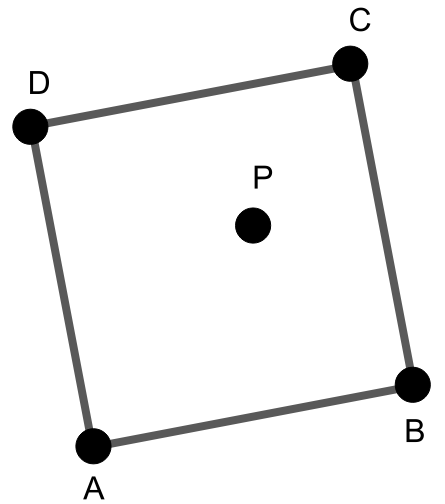
\includegraphics[scale=0.45]{img/quadrado_ponto.png}
    	\end{center}
    	\legend{Fonte: Elaborada pelo autor}
    \end{figure}
     
    Dado um ponto P e um quadrado definido pelos pontos A, B, C e D como o mostrado na figura \autoref{img:quadrado_ponto}, para se determinar se o ponto está dentro do quadrado, a estratégia utilizada passa por dois passos, o primeiro é verificar se o ponto está na região entre as retas $\overline{AB}$ e $\overline{DC}$, o segundo é verificar se o ponto está na região entre as retas $\overline{AD}$ e $\overline{BC}$. Se o ponto estiver nas duas regiões ao mesmo tempo, ele está portanto dentro do quadrado.
    
    \begin{figure}[!htb]
        \caption{\label{img:quadrado_regioes} A figura representa duas regiões em amarelo de um mesmo quadrado, onde caso um ponto estiver ao mesmo tempo nas duas regiões, significa que ele está dentro do quadrado}
    	\begin{center}
            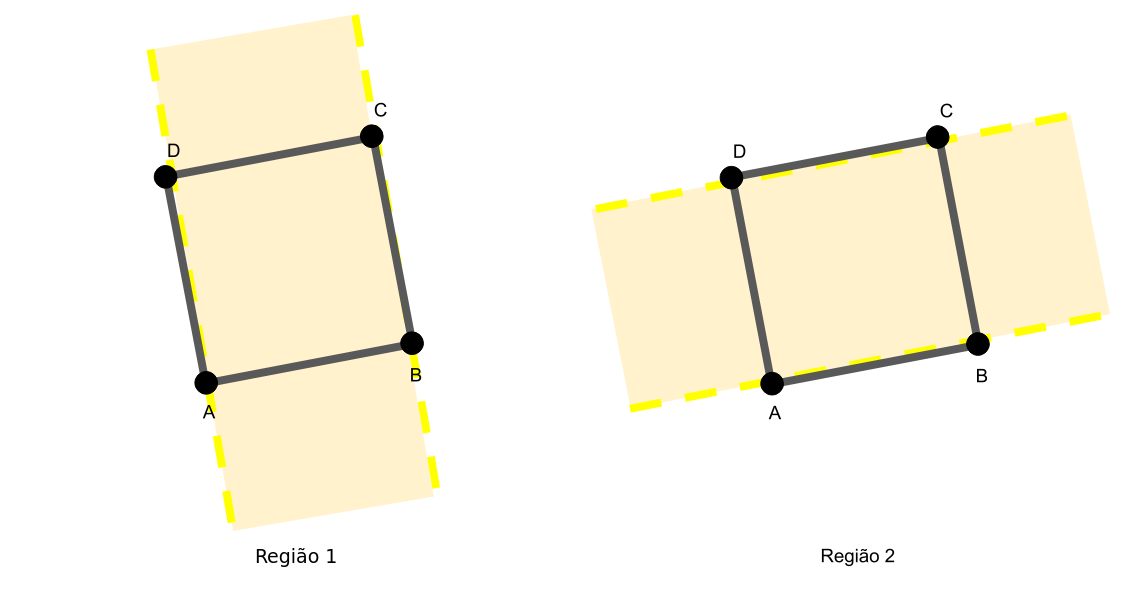
\includegraphics[scale=0.5]{img/quadrado_regioes.png}
    	\end{center}
    	\legend{Fonte: Elaborada pelo autor}
    \end{figure}
    
    Para se determinar se o ponto está dentro da região 1, de acordo com a \autoref{img:quadrado_regioes}, primeiro define-se dois vetores unitários: $\hat{j}$ no sentido do vetor $\overrightarrow{AD}$ e $\hat{k}$ no sentido do vetor $\overrightarrow{AB}$. Então se define dois outros vetores: $\overrightarrow{P_j}$ que é a projeção do vetor $\overrightarrow{AP}$ no vetor $\hat{j}$, e o vetor $\overrightarrow{P_k}$ que é a projeção do vetor $\overrightarrow{AP}$ no vetor $\hat{k}$, como pode-se ver na \autoref{img:quadrado_vetores}.
     
    \begin{figure}[!htb]
        \caption{\label{img:quadrado_vetores} Representação dos vetores utilizados para se determinar se um ponto se encontra dentro de um quadrado}
    	\begin{center}
            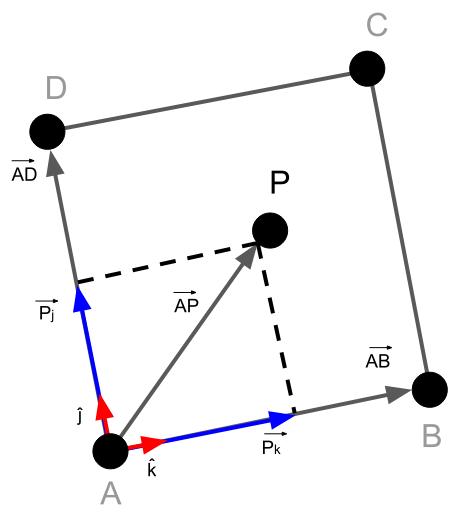
\includegraphics[scale=0.55]{img/quadrado_vetores.png}
    	\end{center}
    	\legend{Fonte: Elaborada pelo autor}
    \end{figure}
    
    Como:
    
    \begin{equation}
        \overrightarrow{AB} = \norm{\overrightarrow{AB}}\cdot \hat{k} + 0 \cdot \hat{j}
    \end{equation}
    
    \begin{equation}
        \overrightarrow{AP} = \norm{\overrightarrow{P_k}} \cdot \hat{k} + \norm{\overrightarrow{P_j}} \cdot \hat{j}
    \end{equation}
    
    Portanto:
    
    \begin{equation}
        \overrightarrow{AB} \cdot \overrightarrow{AP} = \norm{\overrightarrow{AB}} \cdot \norm{\overrightarrow{P_k}} + 0 \cdot \norm{\overrightarrow{P_j}}
    \end{equation}
    
    \begin{equation}
        \label{eq:escalar1}
        \overrightarrow{AB} \cdot \overrightarrow{AP} = \norm{\overrightarrow{AB}} \cdot \norm{\overrightarrow{P_k}}
    \end{equation}
    
    E pode-se afirmar que:
    
    \begin{equation}
        \label{eq:inequacao1}
        0 < \norm{\overrightarrow{AB}} \cdot \norm{\overrightarrow{P_k}} < \norm{\overrightarrow{AB}} \cdot \norm{\overrightarrow{AB}}
    \end{equation}
    
    Se:
    
    \begin{equation}
        \label{eq:condicoes_regiao}
        0 < \norm{\overrightarrow{P_k}} < \norm{\overrightarrow{AB}} \quad ; \quad \norm{\overrightarrow{AB}} > 0
    \end{equation}
    
    Quando as condições na \autoref{eq:condicoes_regiao} são cumpridas, o ponto P está dentro da região 1, ilustrada na \autoref{img:quadrado_regioes}. Se substitui então a \autoref{eq:escalar1} na \autoref{eq:inequacao1}, para se obter:
    
    \begin{equation}
        \label{eq:quadrado_quase_final}
        0 < \overrightarrow{AB} \cdot \overrightarrow{AP} < \norm{\overrightarrow{AB}} \cdot \norm{\overrightarrow{AB}}
    \end{equation}
    
    E como: 
    
    \begin{equation}
        \label{eq:quadrado_regrinha_simples}
        \norm{\overrightarrow{AB}} \cdot \norm{\overrightarrow{AB}} = \overrightarrow{AB} \cdot \overrightarrow{AB}
    \end{equation}
    
    Se substitui a \autoref{eq:quadrado_regrinha_simples} na \autoref{eq:quadrado_quase_final} para se obter:
    
    \begin{equation}
        \label{eq:quadrado_metade_do_caminho_FINAL}
        0 < \overrightarrow{AB} \cdot \overrightarrow{AP} < \overrightarrow{AB} \cdot \overrightarrow{AB}
    \end{equation}
    
    A \autoref{eq:quadrado_metade_do_caminho_FINAL} é a equação utilizada para se determinar se um ponto se encontra dentro da região 1, onde basta que a equação seja satisfeita para que isso ocorra. De modo análogo, pode-se fazer esse mesmo desenvolvimento matemático para chegar à \autoref{eq:quadrado_outra_metade_FINAL}, que determina se um ponto se encontra dentro da região 2.
    
    \begin{equation}
        \label{eq:quadrado_outra_metade_FINAL}
        0 < \overrightarrow{AD} \cdot \overrightarrow{AP} < \overrightarrow{AD} \cdot \overrightarrow{AD}       
    \end{equation}

    Portanto, para se determinar se o ponto está dentro do quadrado, basta verificar se as condições na \autoref{eq:quadrado_metade_do_caminho_FINAL} e \autoref{eq:quadrado_outra_metade_FINAL} são satisfeitas.

\end{alineas}

\subsubsection{Algoritmo do simulador}

Toda vez que a função de atualização da classe \textit{Fisica} é chamada, o simulador calcula a próxima posição em que cada robô e a bola irão estar (considerando o intervalo de tempo desde a última chamada dessa função), então é verificado se ouve alguma colisão e se faz o tratamento adequado dela. Após isso, é atualizada as posições dos robôs e da bola. A seguir se encontra um passo a passo mais detalhado do algoritmo implementado dentro da função de atualização da classe \textit{Fisica}:

\begin{alineas}[leftmargin=0pt, itemindent=20pt, labelwidth=15pt, labelsep=5pt, listparindent=1.25cm, align=left]

\item É feito o cálculo da próxima posição dos robôs.

Para se calcular o ângulo em que o robô estará com a sua frente direcionada ($0^o$ o robô está direcionado para cima no simulador e $180^o$ o robô está direcionado para baixo no simulador) é utilizada a seguinte equação:

\begin{equation}
    \label{eq:algo:angulo_robo}
    \text{Próximo ângulo} = \text{ângulo anterior} \cdot \text{velocidade angular} \cdot \Delta T
\end{equation}

Onde $\Delta T$ representa o intervalo de tempo desde a última vez que a função de atualização foi chamada. As equações \autoref{eq:algo:posx} e \autoref{eq:algo:posy} calculam as próximas posições em X e Y dos robôs com base na sua velocidade linear.

\begin{equation}
    \label{eq:algo:posx}
    \text{Próxima posição em x} = \text{robô}_{pos_x} - \text{sen}(\text{robô}_{ang} \cdot \frac{\pi}{180}) \cdot \text{robô}_{vel} \cdot \Delta T
\end{equation}

\begin{equation}
    \label{eq:algo:posy}
    \text{Próxima posição em y} = \text{robô}_{pos_y} + \text{cos}(\text{robô}_{ang} \cdot \frac{\pi}{180}) \cdot \text{robô}_{vel} \cdot \Delta T
\end{equation}

\item Checa todos os vértices do robô (vértices do quadrado que representa o robô dentro do simulador), se algum deles colidiu com a parte externa do campo.

Essa etapa checa primeiramente a colisão com todas as laterais do campo que estão na posição vertical ou horizontal, para isso se utiliza a técnica (a) da \autoref{cap:calc_colisao}. A seguir se checa se houve colisão com as partes do campo que não estão na posição vertical ou horizontal. Para isso, se utiliza a técnica (b) abordada na \autoref{cap:calc_colisao}.

\item É verificado se alguma trave do gol se encontra dentro do quadrado que representa o robô utilizando-se a técnica de encontrar um ponto dentro de um quadrado descrita na \autoref{cap:calc_colisao}.

\item Checa se algum robô colidiu com outro robô.

Para essa parte do algoritmo, para fins de performance, primeiramente se checa se algum robô se encontra na região de colisão de outro robô. A região de colisão é quando pelo menos um dos vértices do robô, se encontra dentro de um círculo centrado no ponto central do robô e com raio igual à distância entre o ponto central do robô e algum de seus vértices. A \autoref{img:regiao_de_colisao} mostra a região de colisão de um robô, se o vértice de algum outro robô se encontra a região de colisão dele, se considera que esse outro robô essa na região de colisão.

\begin{figure}[!htb]
    \caption{\label{img:regiao_de_colisao}Região de colisão de um robô representada por um círculo vermelho}
	\begin{center}
        
\includegraphics[scale=0.5]{img/zona_de_perigo.png}
	\end{center}
	\legend{Fonte: Elaborada pelo autor}
\end{figure}
 
 Quando um robô se encontra na região de colisão de outro robô, é então verificado se algum dos vértices desses robôs, está colidindo com o outro. Isso é feito utilizando a técnica mostrada na \autoref{cap:calc_colisao} para se determinar se um ponto se encontra dentro de um quadrado.
 
 \item Atualiza a posição de todos os robôs.
 
 Atualiza a posição de todos os robôs que não colidiram para a posição calculada no item (a). Os robôs que sofreram algum tipo de colisão não se movem.
 
 \item Colisão da bola com o robô.
 
 Primeiramente se verifica se a bola se encontra na região de colisão de algum robô. Se a bola está na região de colisão de algum robô, então é checado se a bola colidiu com alguma das arestas do robô. Se a bola colidiu com o robô, então é encontrado o ponto de colisão da bola com o robô, a velocidade relativa do robô naquele ponto de colisão e é somada essa velocidade relativa do ponto de colisão com a velocidade da bola, levando-se em consideração o efeito observado na \autoref{img:reflexao_bola} para se calcular a velocidade resultante da bola.

\item Colisão da bola com o campo.

Verifica-se se a bola colidiu com o campo, se sim, a nova velocidade da bola é calculada, considerando-se o efeito representado na \autoref{img:reflexao_bola}.

\item Atualiza a posição da bola.

% =========================================================================================
\end{alineas}

\subsection{Interface}

Existe uma classe no sistema chamada \textit{Interface} que pode ser vista na \autoref{img:simulador_blocos}, ela tem o proposito de servir como o único meio de comunicação entre o simulador e o resto do sistema, passando informações sobre os robôs e a bola na simulação para o AG e para a RNA quando solicitado e recebendo dados dos mesmos também.

Além de servir como meio de comunicação, essa classe também faz a conversão dos valores de forma conveniente para o simulador e o outros módulos que o utilizarão. Para o treinamento de uma rede neural, é vantajoso que os valores estejam normalizados, isso acarreta em um menor erro de estimação e menor tempo de treinamento necessário \cite{589532}. A normalização adotada foi fazer todos os valores variarem entre 0 e 1, portanto, para a utilização do simulador, as variáveis lidas nele, desde as de posição quanto as de velocidade, estão nesse intervalo. A classe interface traduz esses dados normalizados para dados nas unidades que o simulador trabalha facilitando a comunicação entre os módulos.

\section{Rede Neural Artificial}

Foi implementada uma RNA do tipo perceptron multicamadas (PMC) que consegue se comunicar com o simulador utilizando a classe \textit{Interface}. A RNA atua como a IA de um time de robôs, porém ela pode controlar quantos robôs forem desejados, não se limitando a um time de 3 robôs. 

As entradas da RNA podem ser quaisquer variáveis disponíveis do simulador pela classe \textit{Interface} e as saídas da RNA são a velocidade angular e velocidade linear de cada robô que ela controla.

Ao se criar uma nova RNA, deve-se inserir como parâmetro de entrada como vai ser a sua topologia, ou seja, quantas entradas a RNA vai ter, quantas saídas (duas para cada robô que ela controlar), quantas camadas internas de neurônios ela vai ter e quantos neurônios em cada camada.

As RNAs podem ser salvas em um arquivo após seu treinamento para posterior utilização ou aplicação de uma nova etapa de treinamento. Foi também desenvolvida uma função para ler um arquivo previamente salvo e gerar uma RNA a partir dele.

A RNA sozinha é capaz de dado os valores que estão na sua entrada calcular os valores da saída, porém é necessário atualizar as entradas com os últimos valores calculados pelo simulador, e é necessário inserir os valores calculados pela RNA de volta ao simulador, para realizar essas ações foi criada a classe \textit{FeedForward}. A classe \textit{FeedForward} atualiza as entradas da RNA com os valores do simulador, faz a chamada da função que calcula a saída dela e atualiza o simulador com os valores calculados. A \autoref{img:feedforward} apresenta o fluxo de dados, desde a sua leitura do simulador utilizando a \textit{Interface} pela classe \textit{FeedForward}, até o calculo das próximas ações de cada robô e a inserção dessas informações no simulador.

\begin{figure}[!htb]
    \caption{\label{img:feedforward}Diagrama com o fluxo de dados de cada iteração do \textit{FeedForward}}
	\begin{center}
        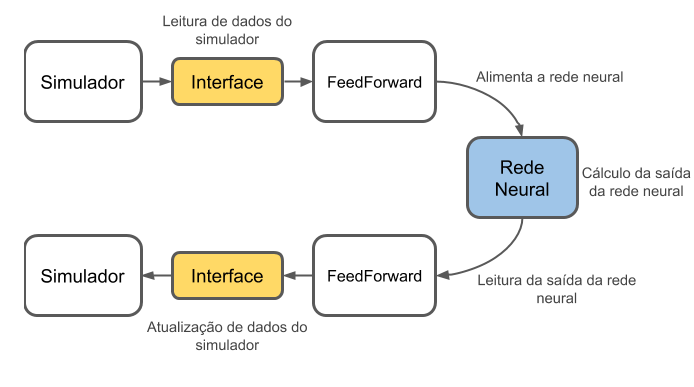
\includegraphics[scale=0.75]{img/blocos_feedforward.png}
	\end{center}
	\legend{Fonte: Elaborada pelo autor}
\end{figure}

\section{Classe \textit{GamePlay}}

Uma das partes centrais do sistema desenvolvido é a classe \textit{GamePlay}, ela é responsável por ditar o ritmo e inicializar o módulos que são necessários para simular uma partida de futebol de robôs, sendo que a partida é definida nesse contexto como o período em que a simulação física dos robôs está ocorrendo, junto com os diversos módulos que interagem com a simulação. Os módulos que interagem com \textit{GamePlay} são as classes: \textit{Fisica}, \textit{Grafico}, \textit{Referee}, \textit{Fitness} e \textit{FeedForward}.

\begin{figure}[!htb]
    \caption{\label{img:gameplay_modulos}Diagrama mostrando as classes que a \textit{GamePlay} controla}
	\begin{center}
        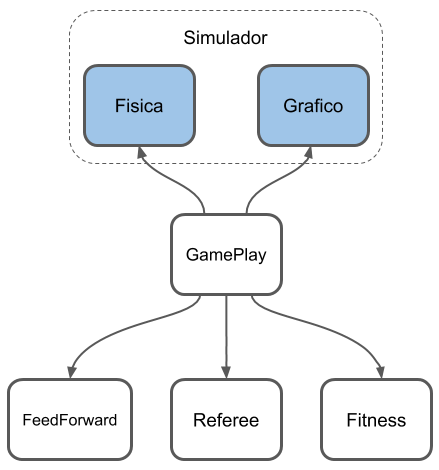
\includegraphics[scale=0.75]{img/blocos_gameplay.png}
	\end{center}
	\legend{Fonte: Elaborada pelo autor}
\end{figure}

A classe \textit{Referee} é responsável por atuar sobre a simulação como se fosse o arbitro de um jogo de futebol, tomando ações que influenciam no jogo quando determinados critérios são atingidos. Exemplos de ações que a classe \textit{Referee} pode tomar são: finalizar uma partida quando o tempo limite de duração se esgota, reiniciar os robôs e a bola para as posições iniciais quando um gol é feito e fazer a contagem de gols e finalizar a partida quando um time atinge determinado número de gols. A classe \textit{Fitness} faz parte do algoritmo evolutivo, ela será descrita com mais detalhes no capítulo~\ref{cap:algoritmo_genetico}.

Tendo acesso e controle de todas as classes ilustradas na \autoref{img:gameplay_modulos} a classe \textit{GamePlay} é utilizada sempre que é necessário simular algo. Ela já possui implementado dentro dela funções para simular uma partida sem a parte gráfica, com a parte gráfica, com apenas um robô, com dois times de três robôs, etc. Dessa forma toda a simulação da partida, e a interação do simulador com as classes da inteligência artificial fica modularizada dentro dela.

\section{\textcolor{blue}{\label{cap:algoritmo_genetico}Algoritmo Genético}}

Foi implementado um algoritmo genético capaz de ensinar uma RNA por meio do ajuste dos pesos de seu neurônio, a realizar determinada ação com os robôs. Para validação do sistema e testes iniciais foi desenvolvida uma IA que faz um robô ir de um ponto a outro do campo.

Existem quatro classes que são importantes para o AG que foi implementado: \textit{EvolutionControl}, \textit{Crossover} e \textit{Fitness}. A classe \textit{Fitness} acompanha cada iteração da simulação, ela é uma das partes mais importantes na definição do desempenho da rede neural, pois ela da pontos de aptidão para a rede neural a cada iteração da simulação de acordo com o modo que ela foi programada, e esses pontos influenciam diretamente em quais características serão passadas para a próxima geração do AG e quais serão excluídas. A classe \textit{Crossover} contém funções responsáveis pela reprodução e mutação dos indivíduos do AG. A classe \textit{EvolutionControl} controla todo o AG. Um fluxograma mostrando as relações entre as principais classes referentes ao AG encontra-se na \autoref{img:algoritmo_genetico_compacto}.

\begin{figure}[!htb]
    \caption{\label{img:algoritmo_genetico_compacto}Diagrama mostrando as interações entre as principais classes relacionadas ao AG}
	\begin{center}
        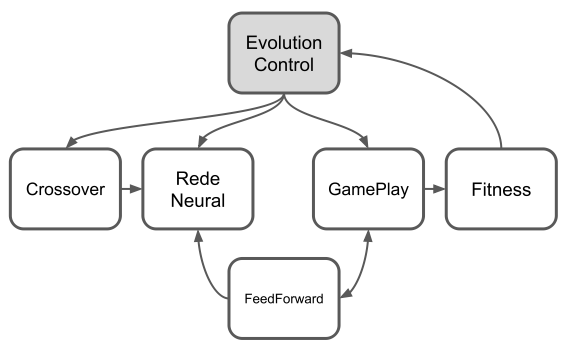
\includegraphics[scale=0.75]{img/ag_compacto.png}
	\end{center}
	\legend{Fonte: Elaborada pelo autor}
\end{figure}

Foram feitos vários testes diferentes com o AG a fim de se conseguir treinar uma RNA para controlar um robô e fazer ele se mover de um ponto a outro do mapa

%====================================
\textcolor{red}{
\begin{itemize}
    \item explicar como é a estrutura do AG, talvez tomar como base o diagrama de blocos q ta no power point
    \item explica cada ponto do diagrama e como eles se relacionam
    \item explicar como isso pode ser utilizado por outra pessoa para treinar uma IA diferente (criar crossover novo, mudar o fitness, etc)
\end{itemize}
}

\textcolor{blue}{
Explicar todas as classes que eu criei para o AG funcionar e como elas se relacionam entre si. No qual o usuário teria que modificar para o AG treinar o que ele quiser
}

\subsection{População Inicial}
\subsection{Função de Aptidão}
\subsection{Seleção do mais Apto}
\subsection{Crossover}
\subsection{Predação}




\section{\textcolor{blue}{Implementação}}
\textcolor{red}{Explicar como eu juntei o simulador, a rede neural artificial e o algoritmo evolutivo e fiz os treinamentos.}


